% !TeX spellcheck = en_GB
\section{Wednesday, \SI{21}{\dec}}\label{sec:2112}

%%% short info on Mondays general weather
At the Haukeliseter measurement site was precipitation observed by the double fence from \SI{10}{\UTC} and last almost continuously through the event. The precipitation amount was moderately and Norway was located within a cold air section (\Cref{sec:largeScale}). 

%%%%%%%%%%%%%%%%%%%%%%%%%%%%%%%%%%%%%%%%%%%%%%%%%%%%%%%%%%%%%%%%%%%%%%%%%%
%%%%%%%%% surface obs %%%%%%%%%%%%%%
\subsection{Surface accumulation}
The surface accumulation at the ground showed a good agreement between retrieved snowfall amount, MEPS precipitation amount, and the reference frame of the double fence gauge. Since MEPS had some outlier ensemble members a box-whisker-plot is been provided.
%%% image surface MEPS boxplot %%%%%%%%%%%%%%%%%%%%%%%%%%%%%%%%%%%%%
\begin{figure}[t]
	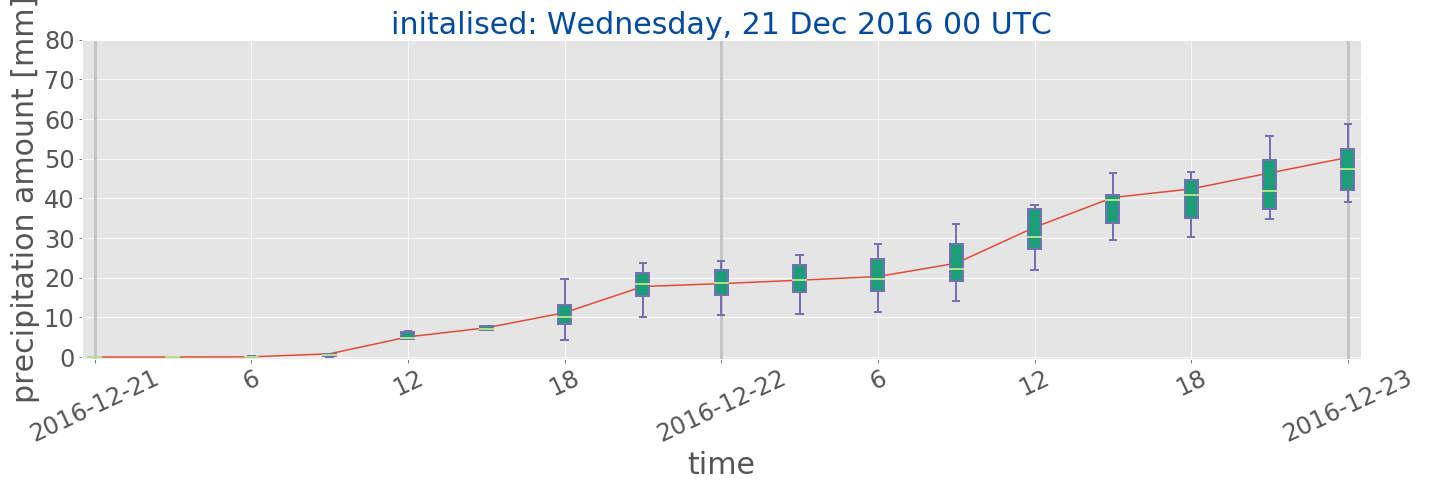
\includegraphics[width=\textwidth]{./fig_boxplot_sfc/20161221_0}
	\caption{Box-whisker-plot of the ten ensemble members of MEPS. Red line indicating the ensemble mean, lower and upper whisker the 25th and 75th percentile, respectively. Light green shows the median of all members and the box represents the middle \SI{50}{\percent} of scores of the precipitation.}\label{fig:boxplt21}
\end{figure}
%%%%%%%%%%%%%%%%%%%%%%%%%%%%%%%%%%%%%%%%%%%%%%%%%%%%%%%%%%%%%%%%%%%%%%%%%%
The box-whisker-plot in \Cref{fig:boxplt21} shows the distribution of the ten ensemble members. In the first \SI{15}{\hour} of the forecast time agree all members well, since the box and whiskers are small. With increasing forecast time, increases the uncertainty. After \SI{30}{\hour} is the ensemble mean slightly higher than the median of the data. In general can the surface forecast be trusted since the values of the ensemble members are well distributed around the mean.
%%%%%%%%%%%%%%%%%%%%%%%%%%%%%%%%%%%%%%%%%%%%%%%%%%%%%%%%%%%%%%%%%%%%%%%%%%
\textcolor{red}{DISCUSSION! The observations from \Cref{fig:SWC21} have shown, that south easterly wind is associated with up-slope storms. If west wind was observed the MRR reflectivity showed patterns of pulsing with a change of intense precipitation to weaker precipitation. West wind is one of the main wind directions at Haukeliseter (\Cref{sec:int:dec_obs})   }
%%%%%%%%%%%%%%%%%%%%%%%%%%%%%%%%%%%%%%%%%%%%%%%%%%%%%%%%%%%%%%%%%%%%%%%%%%
%%%%%%%%% vertical obs %%%%%%%%%%%%%%
\subsection{Vertical snowfall observations}\label{sec:vertEM09:2112}
% %%% image SWP %%%%%%%%%%%%%%%%%%%%%%%%%%%%%%%%%%%%%
\begin{figure}[t]
	\centering
	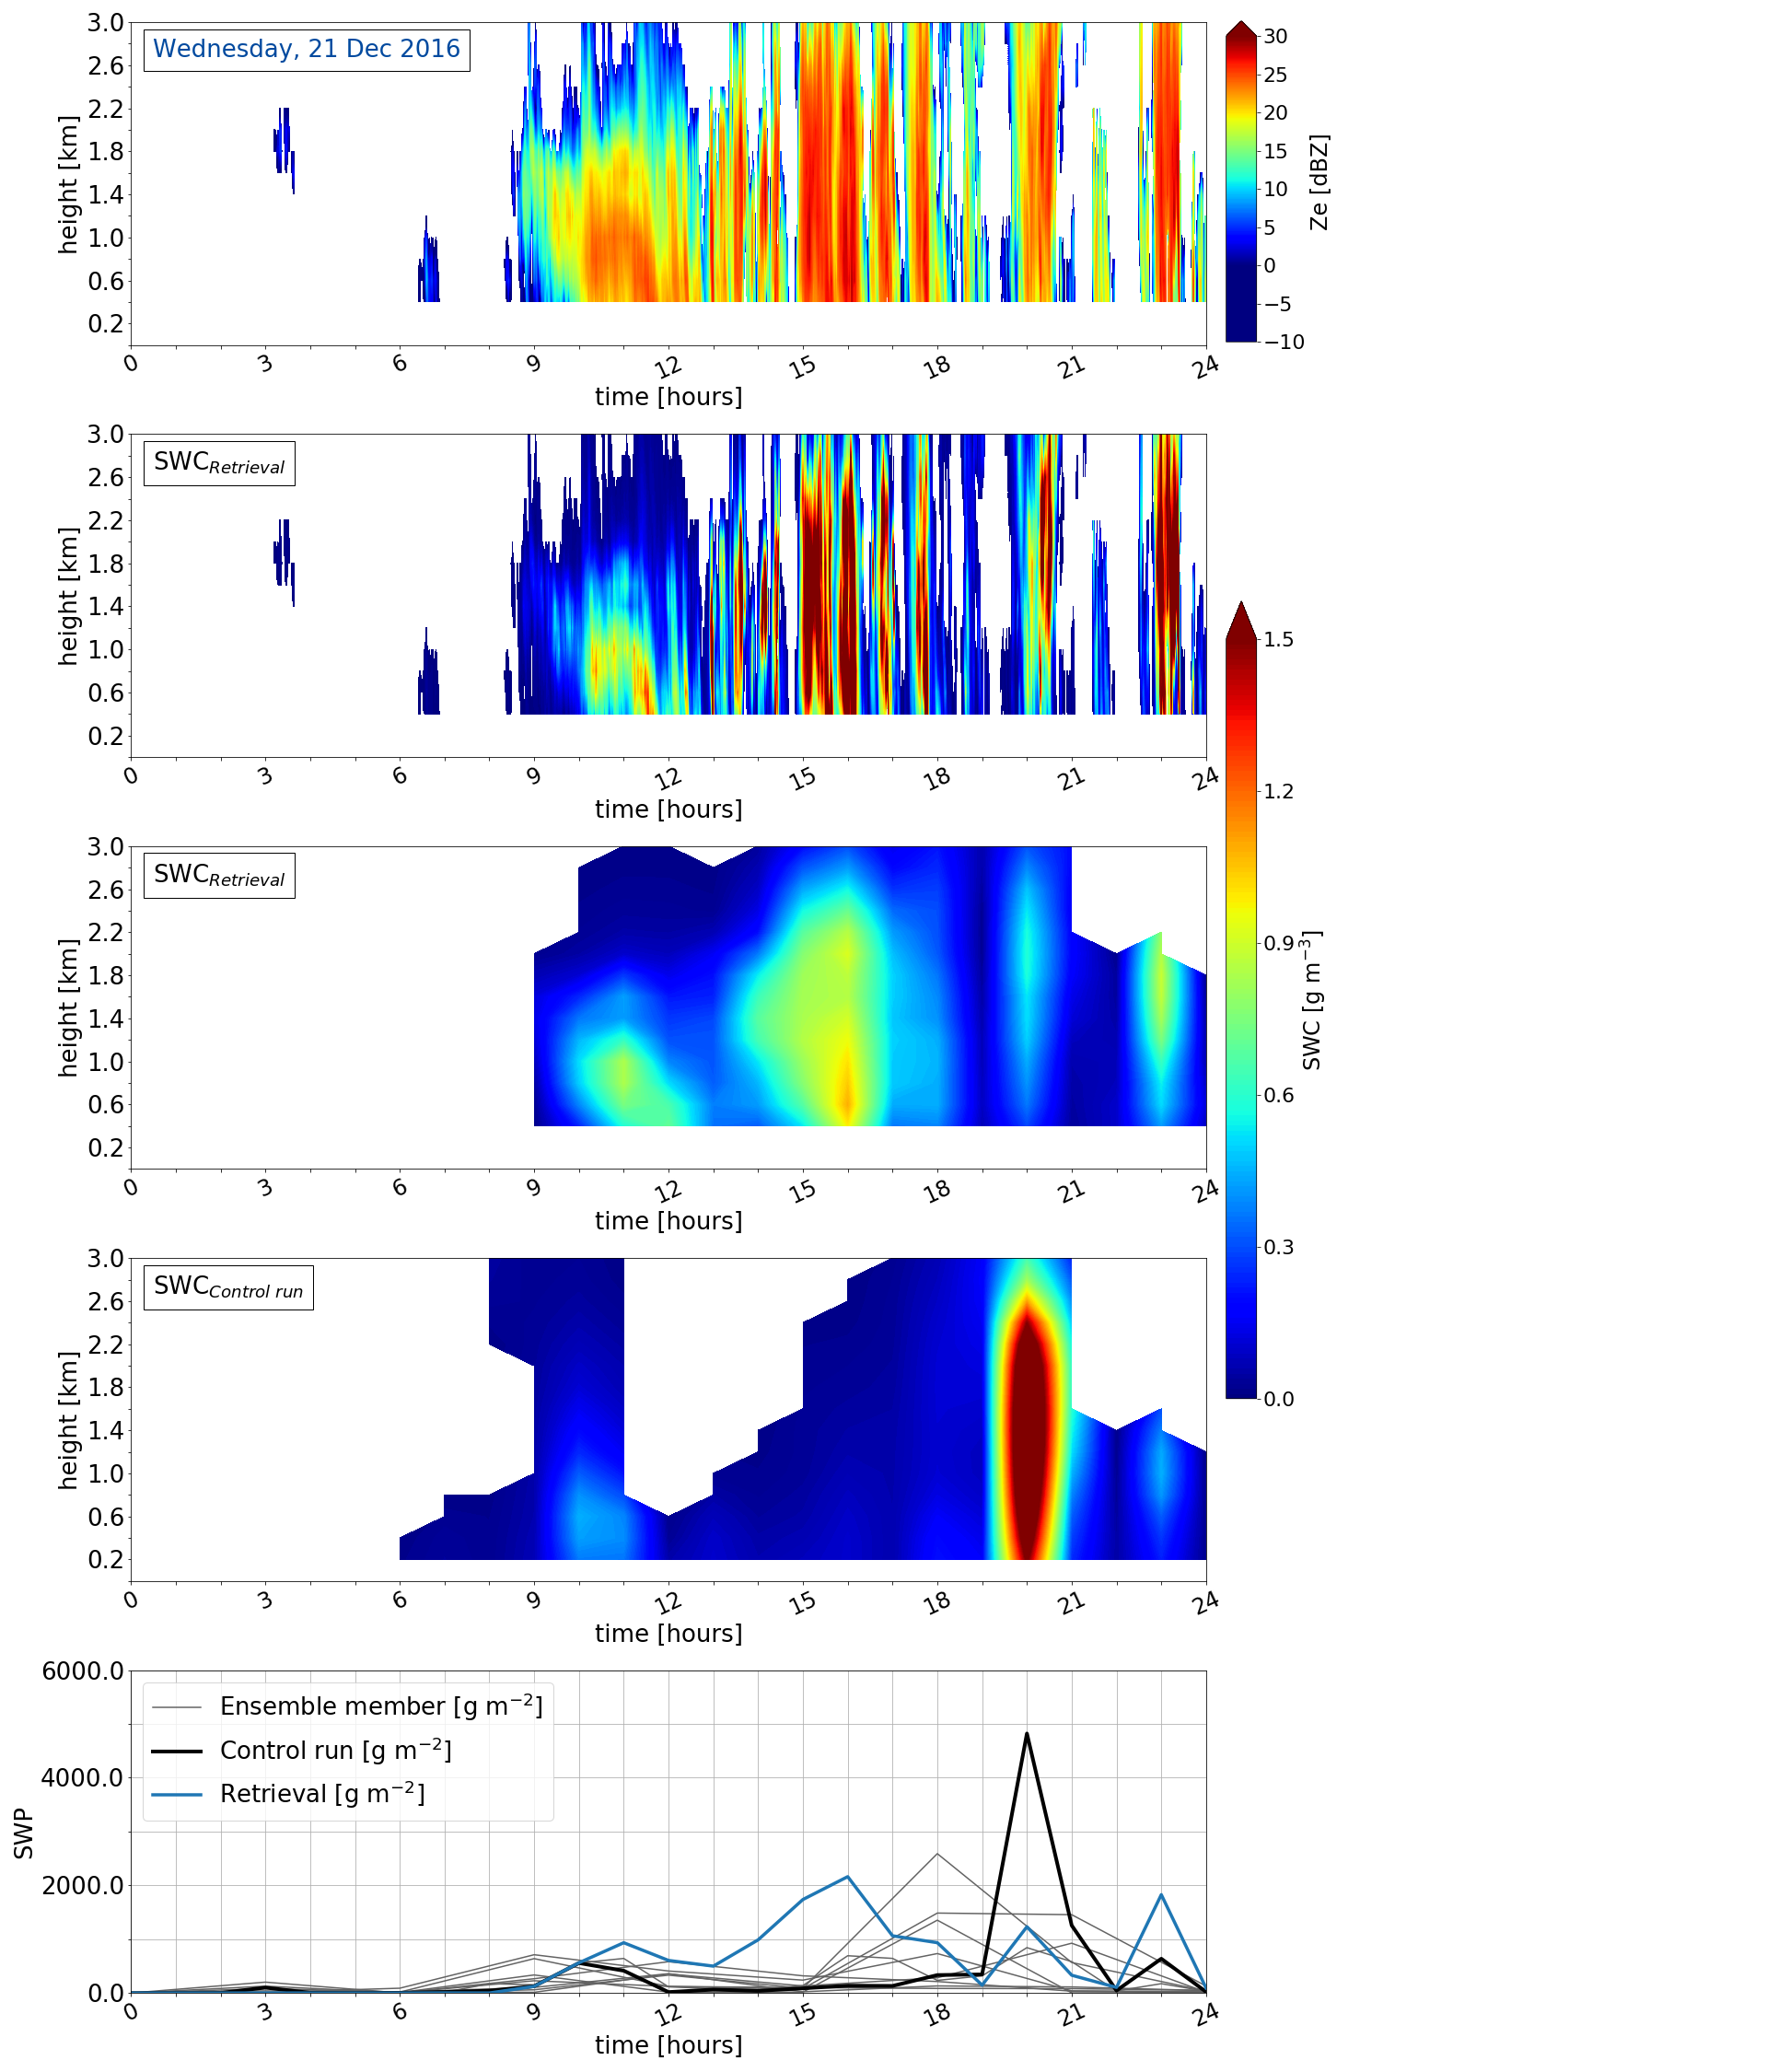
\includegraphics[trim={0.4cm .4cm 31.3cm 63.5cm},clip,width=\textwidth]{./fig_SWC/20161221}
	\caption{}\label{fig:SWP21}
\end{figure}
%%%%%%%%%%%%%%%%%%%%%%%%%%%%%%%%%%%%%%%%%%%%%%%%%%%%%%%%%%%%%%%%%%%%%%%%%%
It shows from the SWP image in \Cref{fig:SWP21}, that the deterministic forecast of MEPS (black line) dominates. Most of the other ensemble members (grey line) prognoses the daily maximum snowfall amount two hours earlier than the deterministic forecast. The blue, dashed line, indicating the ensemble mean SWP shows the weakening of the snowfall amount when taking the average of all ten ensemble members with a maximum value at \SI{20}{\UTC}. By comparing the orange line (SWP from the retrieval) and the blue, dashed line it shows, that the ensemble mean value of MEPS gets closer to the observed one, \SIlist{2833; 2162}{\SWP} respectively.
%
% %%% image ensemble member 0-9 %%%%%%%%%%%%%%%%%%%%%%%%%%%%%%%%%%%%%
\begin{figure}[t]
	\centering
	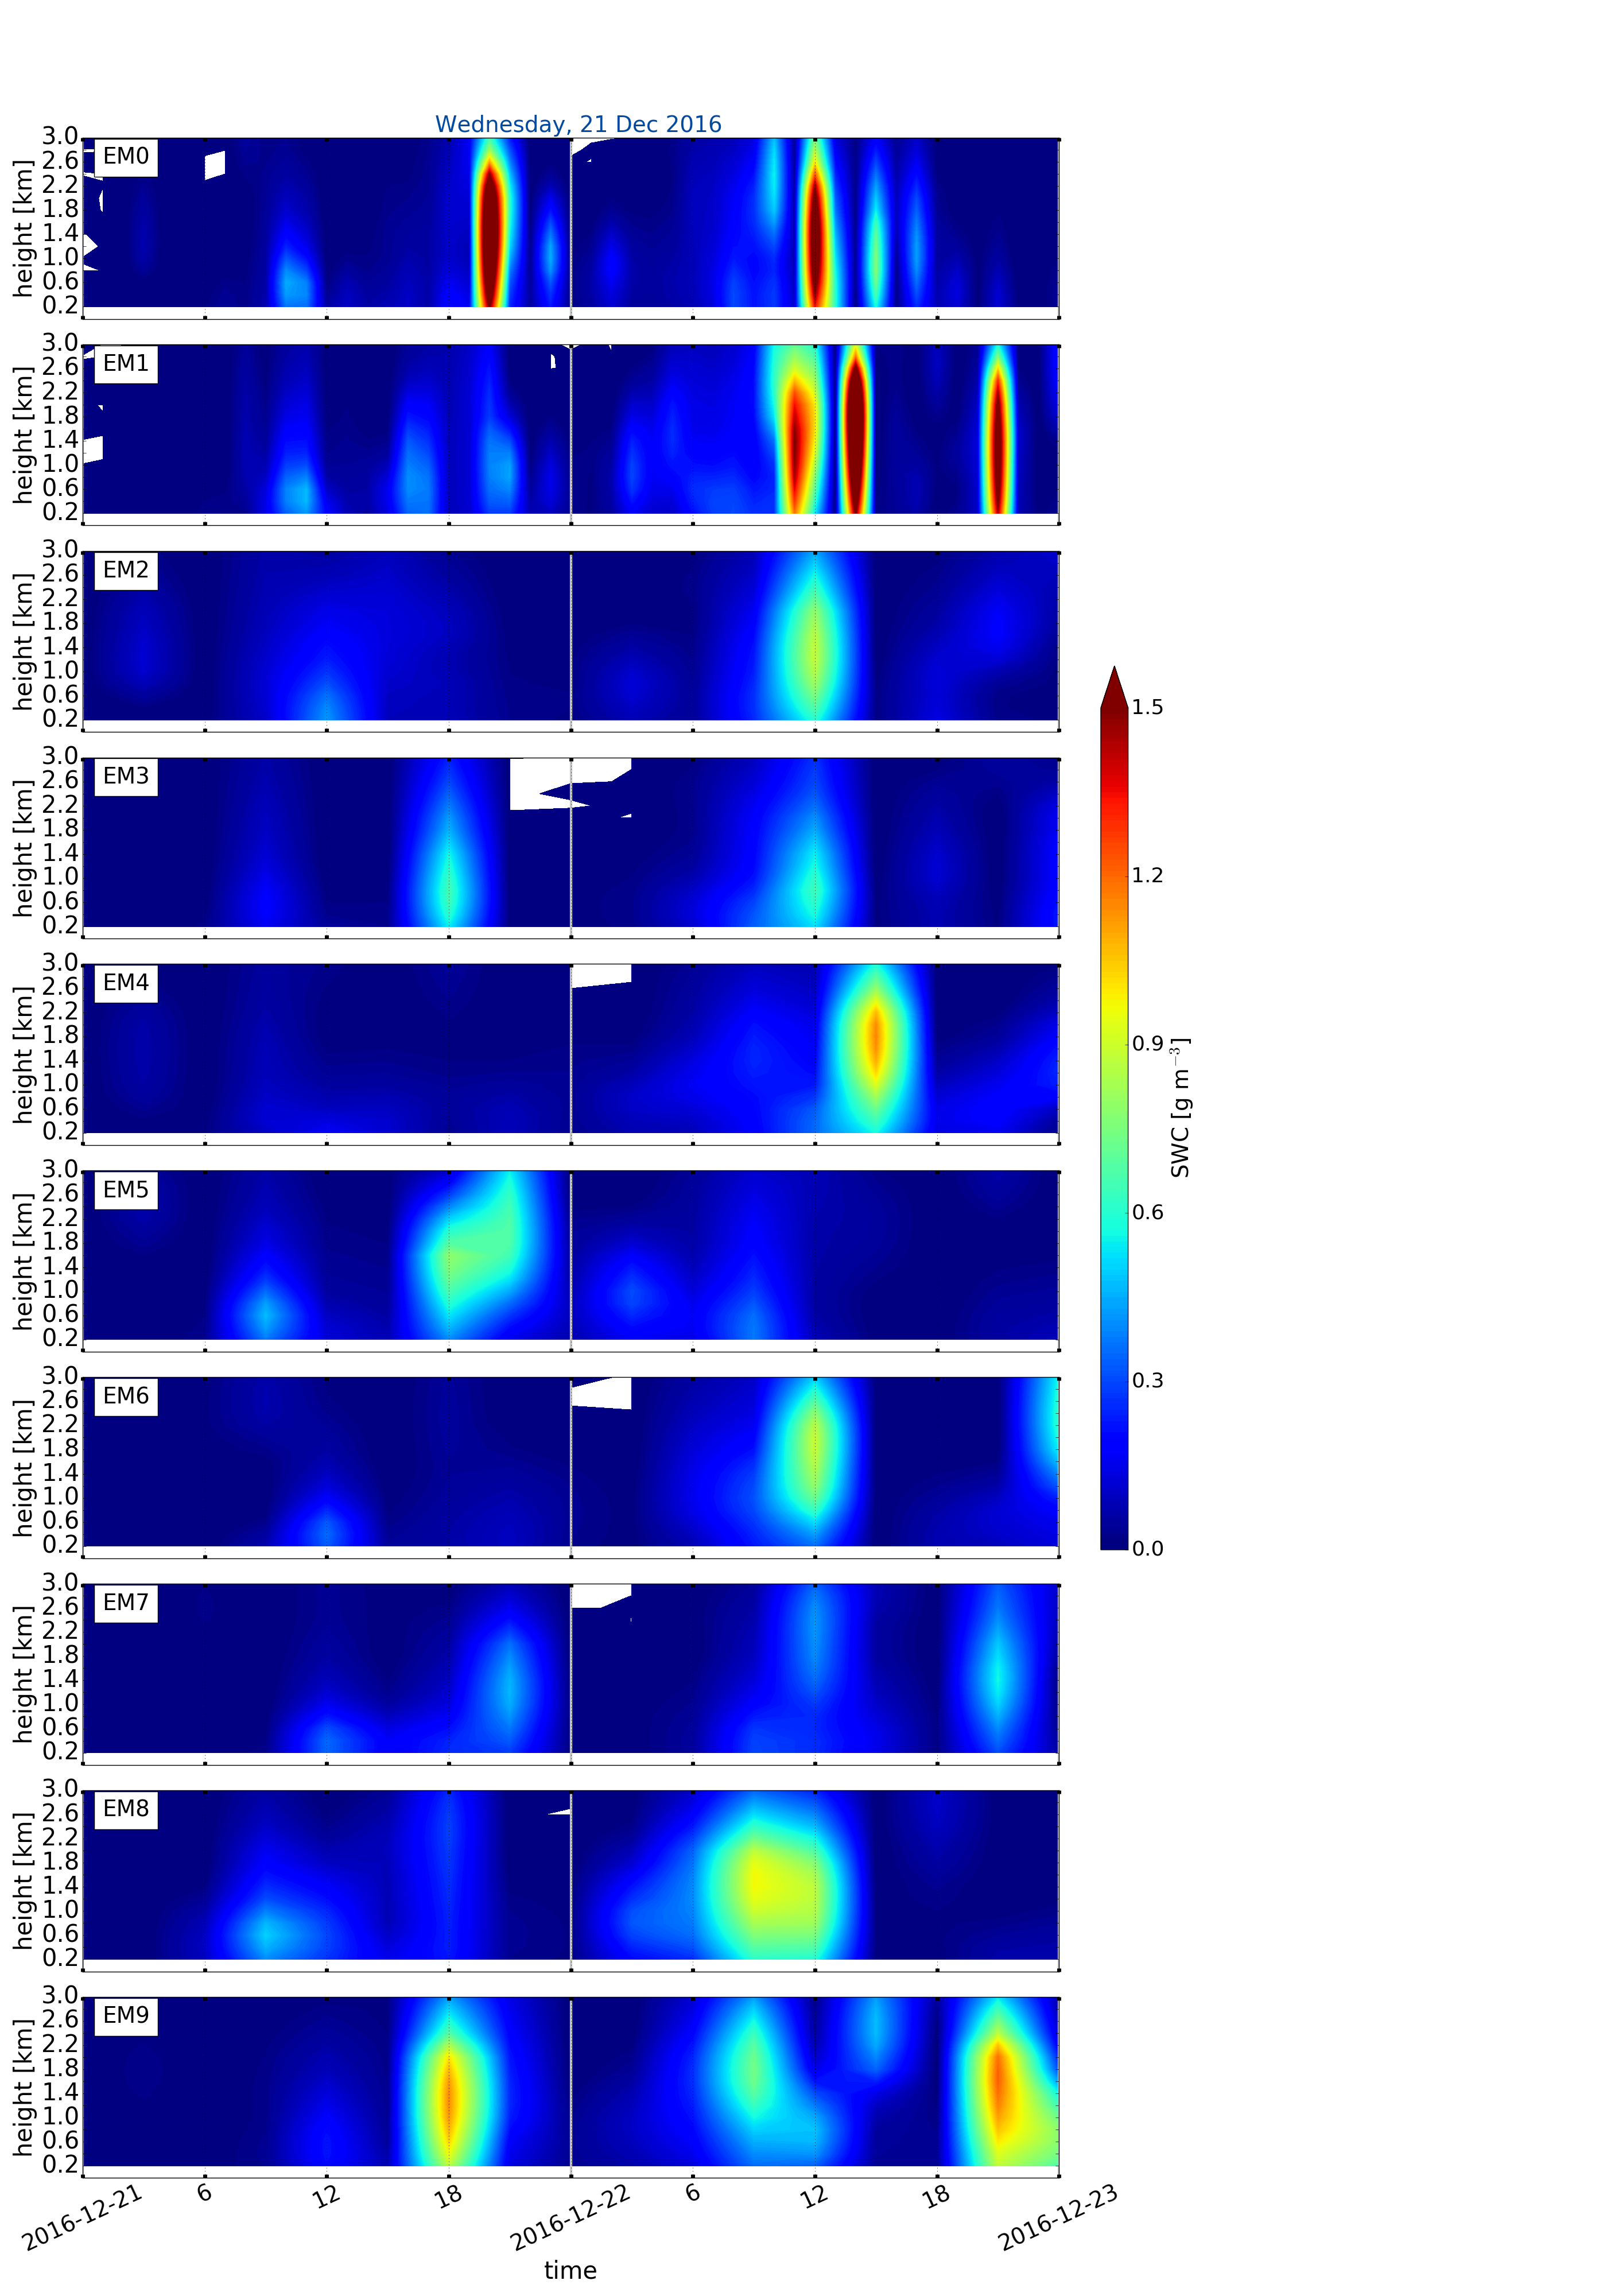
\includegraphics[trim={0cm 0cm 18.3cm 5.1cm},clip,width=0.8\textwidth]{./fig_09EM/20161221}
	\caption{SWC of all ensemble members initialised Wednesday, \SI{21}{\dec} at 0\SI{0}{\UTC} forecast for \SI{48}{\hour}.}\label{fig:EM09_21}
\end{figure}
%%%%%%%%%%%%%%%%%%%%%%%%%%%%%%%%%%%%%%%%%%%%%%%%%%%%%%%%%%%%%%%%%%%%%%%%%%
%
\textcolor{red}{DISCUSSION! Why does MEPS not catch that peak at \SI{16}{\UTC}? Maybe because it is too close to the convective storm. Also, Why is the control so high compared to the perturbed members? It catches the convective part when also a little weak. Most of the ensemble members would have caught it around \SI{9}{\UTC}. One ensemble member has predicted a high value of SWC at \SI{18}{\UTC}, compare to \Cref{fig:EM09_21}.}
% %
\newline \noindent
The vertical temperature profile performed with MEPS in \Cref{fig:meps_sound_20} and \ref{fig:meps_sound_21}, shows that an initialisation \SI{36}{\hour} prior to the event would give a cloud with height up to \SI{3}{\km}, as observed in \Cref{fig:SWC21} first panel. An initialisation closer to the occurrence of the storm shows, that MEPS underestimates the intensity and height of the storm (\Cref{fig:meps_sound_21}).
%
%%% image sounding MEPS %%%%%%%%%%%%%%%%%%%%%%%%%%%%%%%%%%%%%
% !TeX spellcheck = en_GB
\begin{figure}
	\centering
	\begin{subfigure}[b]{0.49\textwidth}
		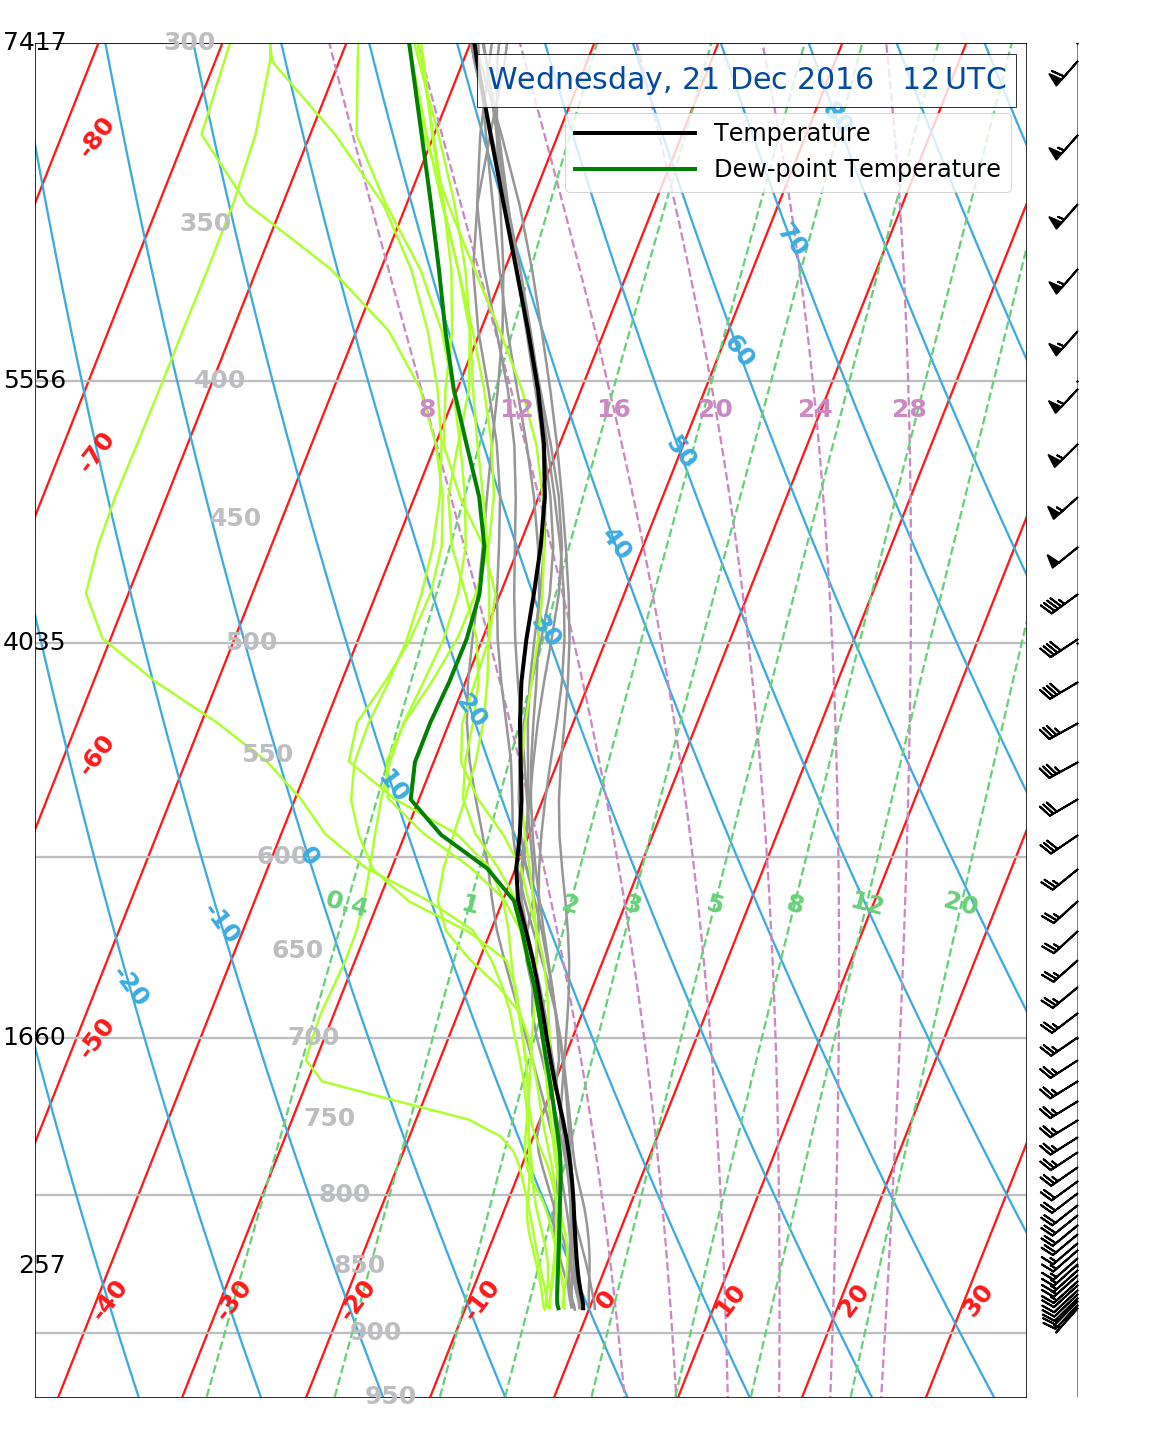
\includegraphics[width=\textwidth]{./fig_Sounding/20161220_36}
		\caption{}\label{fig:meps_sound_20}
	\end{subfigure}
	\begin{subfigure}[b]{0.49\textwidth}
		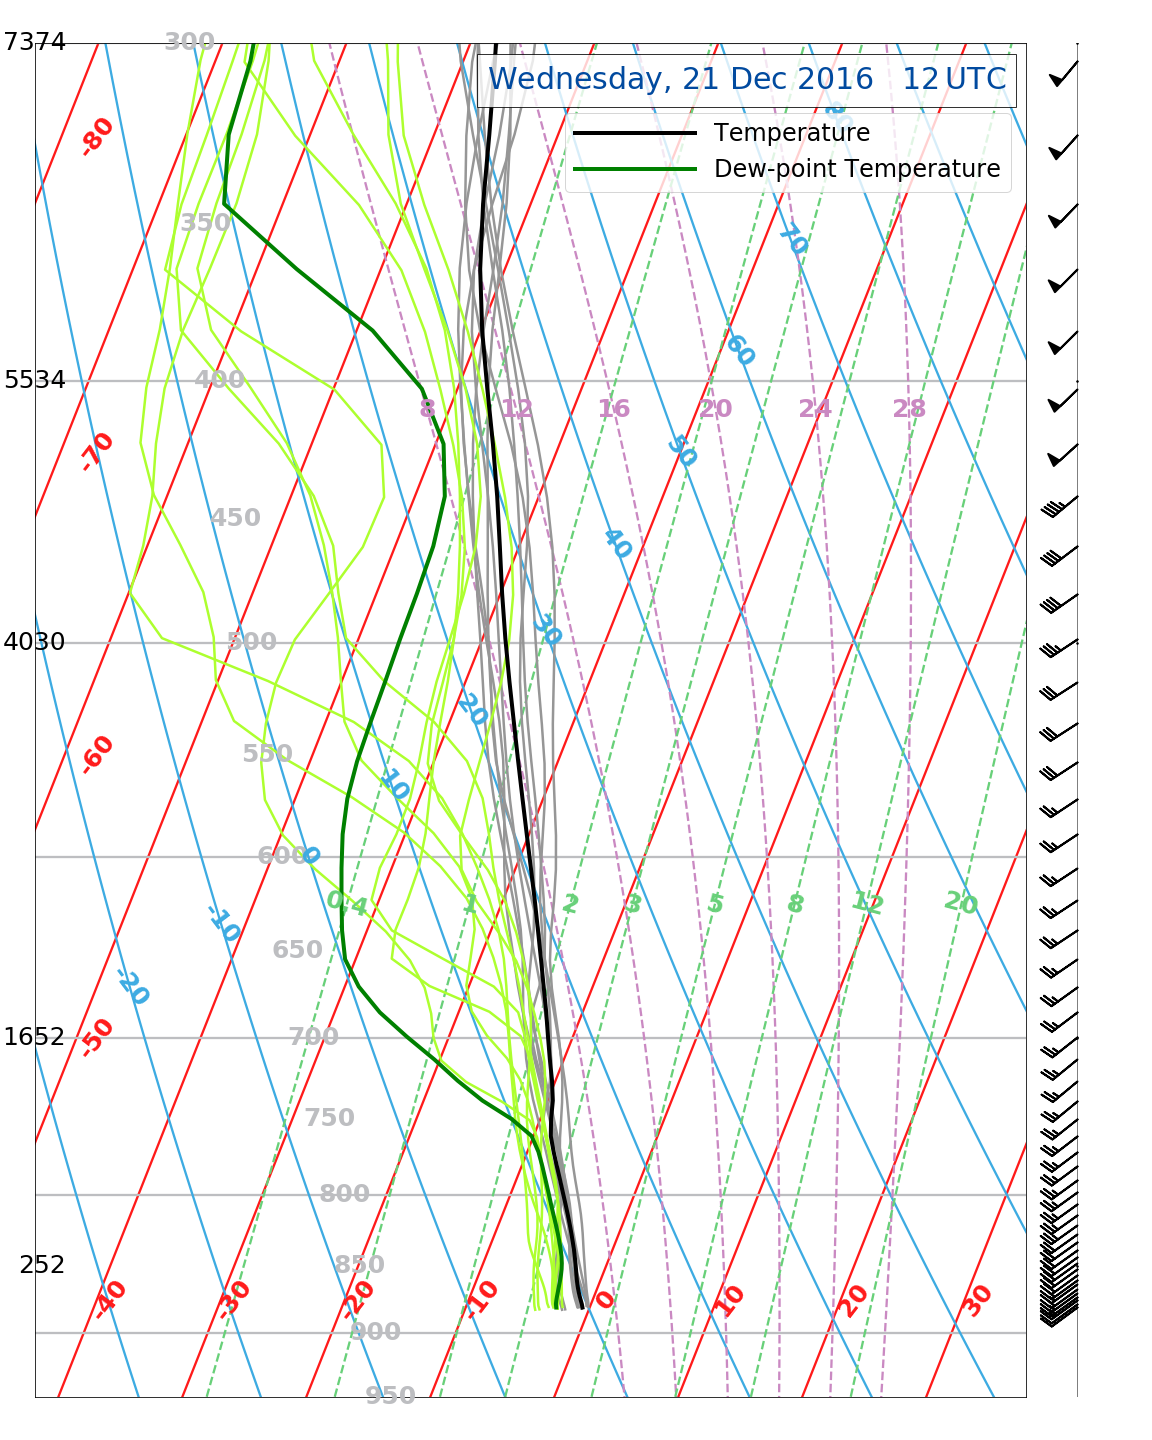
\includegraphics[width=\textwidth]{./fig_Sounding/20161221_12}
		\caption{}\label{fig:meps_sound_21}
	\end{subfigure}
	\caption{Vertical temperature profiles produced with MEPS. \protect{\subref{fig:meps_sound_20}} is initialised: Tuesday, \SI{20}{\dec} \SI{00}{\UTC}. \protect{\subref{fig:meps_sound_21}} is initialised: Wednesday, \SI{21}{\dec} \SI{00}{\UTC}.}
\end{figure}
%%%%%%%%%%%%%%%%%%%%%%%%%%%%%%%%%%%%%%%%%%%%%%%%%%%%%%%%%%%%%%%%%%%%%%%%%%
\textcolor{red}{DISCUSSION! Bring all into relation with the coefficient of variation.}

